We will now consider semigroupoid endowed with topologies which are compatible with their algebraic structures. In general, a (partial) algebraic structure $\mathscr{A}$ consists of families $\mathscr{A}_0$ of sets and $\mathscr{A}_1$ of partial functions between sets in $\mathscr{A}_0$, and $\mathscr{A}$ is said to be \emph{topological} if all sets in $\mathscr{A}_0$ are endowed with topologies, and all functions in $\mathscr{A}_1$ are continuous. The homomorphisms between such structure are also assumed to be continuous. This applies, in particular, to graphs and (Exel/graphed/inverse) semigroupoids. We write the following definitions in full for the sake of completeness.

\begin{definition}
A \emph{topological graph} is a graph $(G^{(0)},G,\so,\ra)$, such that $G^{(0)}$ and $G$ are endowed with topologies making $\so$ and $\ra$ continuous.

A \emph{topological} (Exel) semigroupoid is a semigroupoid $\Lambda$ endowed with some topology which makes the product continuous (where $\Lambda^{[2]}$ is endowed with the product topology of $\Lambda\times\Lambda$).

A topological graphed semigroupoid is a graphed semigroupoid which is both a topological graph and a topological semigroupoid.
\end{definition}

\begin{definition}
A \emph{topological inverse semigroupoid} is an inverse semigroupoid $\mathcal{S}$ which is a topological graphed semigroupoid, and such that the inverse map $(\ )^*\colon\mathcal{S}\to\mathcal{S}$, $s\mapsto s^*$, is continuous.
\end{definition}

Note that since $(\ )^*\circ (\ )^*=\id_{\mathcal{S}}$, then $(\ )^*$ being continuous implies that it is a homeomorphism.

\begin{definition}\label{def:etaleinversesemigroupoid}
A topological inverse semigroupoid $\mathcal{S}$ is \emph{étale} if the source map $\so\colon\mathcal{S}\to\mathcal{S}^{(0)}$ is a local homeomorphism. (Equivalently, the range map $\ra=\so\circ(\ )^*$ is a local homeomorphism.)
\end{definition}

\begin{denv*}{Remark}
As in \cite{MR2304314}, recall that a topological groupoid $\mathcal{G}$ is \emph{étale} if the source map $\so\colon a\mapsto a^{-1}a$ is a local homeomorphism from $\mathcal{G}$ to $\mathcal{G}^{(0)}=\so(\mathcal{G})$, where \emph{$\mathcal{G}^{(0)}$ is endowed with the subspace topology of $\mathcal{G}$}. It is not immediately clear that this coincides with the notion in Definition \ref{def:etaleinversesemigroupoid} since for étale semigroupoids we do not assume $\mathcal{S}^{(0)}$ to even be a subset of $\mathcal{S}$.

Corollary \ref{cor:propertiesopeninversesemigroupoid} below deals with this: Suppose $\mathcal{G}$ is a topological groupoid, étale in the sense of \ref{def:etaleinversesemigroupoid}. Let $\tau$ be the topology of $\mathcal{G}$, $\tau|_{\mathcal{G}^{(0)}}$ ist restriction to $\mathcal{G}^{(0)}$, and $\eta$ the topology of $\mathcal{G}^{(0)}$. By \ref{cor:propertiesopeninversesemigroupoid}\ref{cor:propertiesopeninversesemigroupoid1}, $E(\mathcal{G})=\mathcal{G}^{(0)}$ is open in $\mathcal{G}$. The source map on $\mathcal{G}^{(0)}$ is simply the identity map $(\mathcal{G}^{(0)},\tau|_{\mathcal{G}^{(0)}})\to(\mathcal{G}^{(0)},\eta)$, and it is a bijective (local) homeomorphism, hence $\tau|_{\mathcal{G}^{(0)}}=\eta$.
\end{denv*}

Homomorphisms of topological semigroupoids are always assumed to be continuous. A homomorphism $\phi=(\phi^{(0)},\phi^{(1)})\colon G\to H$ of topological graphs is continuous in the sense that $\phi^{(0)}$ and $\phi^{(1)}$ are continuous. When dealing with topological graphed semigroupoids this is a condition which we need to require, but when dealing with étale inverse semigroupoids, continuity of the ``arrow map'' actually implies continuity of the ``vertex map''. For this we recall a fact from the general theory of étale spaces.

Suppose that $\pi_i\colon X_i^{(1)}\to X_i^{(0)}$ ($i=1,2$) are continuous bundles,  and that $f=(f^{(0)},f^{(1)})\colon\pi_1\to\pi_2$ is a bundle homomorphism (possibly discontinuous a priori). Suppose further that $f^{(1)}$ is continuous and that $\pi_1$ is open (and surjective). Then $f^{(0)}$ is continuous. Indeed, since $\pi_1$ is open and surjective then $X_1^{(0)}$ is endowed with the the quotient (final) topology that $\pi_1$ induces. We have the commutative square
\[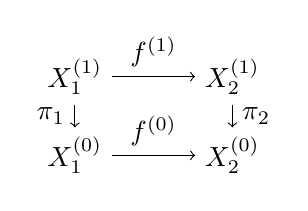
\begin{tikzpicture}
\node (X11) at (0,0) {$X_1^{(1)}$};
\node (X10) at ([shift={+(0,-1)}]X11) {$X_1^{(0)}$};
\node (X21) at ([shift={+(2,0)}]X11) {$X_2^{(1)}$};
\node (X20) at ([shift={+(0,-1)}]X21) {$X_2^{(0)}$};
\draw[->] (X11)--(X21) node[midway,above] {$f^{(1)}$};
\draw[->] (X11)--(X10) node[midway,left] {$\pi_1$};
\draw[->] (X21)--(X20) node[midway,right] {$\pi_2$};
\draw[->] (X10)--(X20) node[midway,above] {$f^{(0)}$};
\end{tikzpicture}\]
which implies that $f^{(0)}$ is the quotient map induced from the continuous map $\pi_2\circ f^{(1)}$, and is therefore continuous.

We thus apply the fact above with the bundle induced by the source maps of graphed semigroupoids, and in conjunction with Corollary \ref{cor:graphedhomomorphisminducesvertexmap} to obtain the result below:

\begin{corollary}
Suppose that $\phi\colon\mathcal{S}\to\mathcal{T}$ is a continuous homomorphism between topological inverse semigroupoids and that $\mathcal{S}$ is étale. Then there exists a unique continuous map $\phi^{(0)}\colon\mathcal{S}^{(0)}\to\mathcal{T}^{(0)}$ for which $(\phi^{(0)},\phi)$ is a graphed semigroupoid homomorphism.
\end{corollary}

A \emph{bisection} of a graphed semigroupoid $\mathcal{S}$ is a subset $U\subseteq\mathcal{S}$ such that the source and range maps are injective on $U$. We denote by $\mathbf{B}(\mathcal{S})$ the set of all open bisections of an étale inverse semigroupoid $\mathcal{S}$. If $U\in\mathbf{B}(\mathcal{S})$, then the source and range maps restrict to homeomorphisms from $U$ onto open subsets of $\mathcal{S}^{(0)}$. Moreover, $\mathbf{B}(\mathcal{S})$ is a basis for the topology of $\mathcal{S}$.

\begin{proposition}\label{prop:productmapisopen}
If $\mathcal{S}$ is an étale inverse semigroupoid then the product map $\mu\colon\mathcal{S}^{(2)}\to\mathcal{S}$ is open.
\end{proposition}
\begin{proof}
We follow the proof of \cite[1.3.11]{cordeirothesis}: Let $\pi\colon \mathcal{S}^{(2)}\to\mathcal{S}$ be the projection $\pi(a,b)=a$. We prove that $\pi$ is open. If $A,B\in\mathbf{B}(\mathcal{S})$, then $\pi((A\times B)\cap \mathcal{S}^{(2)})=A\cap \so^{-1}(\ra(B))$. Since $\ra(B)$ is open in $\mathcal{S}^{(0)}$ and $\so$ is continuous, then $\pi((A\times B)\cap \mathcal{S}^{(2)})$ is open in $\mathcal{S}$. This proves that $\pi$ is open, as $\mathbf{B}(\mathcal{S})$ is a basis for $\mathcal{S}$. Moreover, $\pi$ is injective on $(A\times B)\cap\mathcal{S}^{(2)}$, because the range map is injective on $B$. Therefore, $\pi$ is a locally injective open continuous map, that is, a local homeomorphism.

Since $\ra\circ\pi=\ra\circ\mu$ on $\mathcal{S}^{(2)}$ and both $\ra$ and $\pi$ are local homeomorphisms, then $\mu$ is a local homeomorphism as well.\qedhere
\end{proof}

We thus make $\mathbf{B}(\mathcal{S})$ into a semigroup with the usual product of sets: for all $A,B\in\mathbf{B}(\mathcal{S})$,
\[AB=\left\{ab:(a,b)\in (A\times B)\cap \mathcal{S}^{(2)}\right\}.\]
Then $\mathbf{B}(\mathcal{S})$ is, in fact, an inverse semigroup. However, we are not able to recover the semigroupoid $\mathcal{S}$ from $\mathbf{B}(\mathcal{S})$ alone, since the canonical order of $\mathbf{B}(\mathcal{S})$ does not correspond to set inclusion. We have
\[A\leq B\iff A=BA^*A\iff\text{for all }a\in A\text{ there exists }b\in B\text{ such that }a\leq b.\]

In Section \ref{sec:duality}, we will prove that an inverse semigroupoid $\mathcal{S}$ may be recovered from $\mathbf{B}(\mathcal{S})$ and set inclusion $\subseteq$.

We finish this section by mentioning a few simple, but nevertheless important, consequences of Proposition \ref{prop:productmapisopen}.

\begin{corollary}\label{cor:propertiesopeninversesemigroupoid}
Let $\mathcal{S}$ be an étale inverse semigroupoid. Then
\begin{enumerate}[label=(\alph*)]
    \item\label{cor:propertiesopeninversesemigroupoid1} $E(\mathcal{S})$ is open in  $\mathcal{S}$;
    \item\label{cor:propertiesopeninversesemigroupoid2} For all open $A\subseteq \mathcal{S}$, the \emph{upper} and \emph{lower closures} \[A^{\uparrow,\leq}=\left\{b\in\mathcal{S}:b\geq a\text{ for some }a\in A\right\}\quad\text{and}\quad A^{\downarrow,\leq}=\left\{b\in\mathcal{S}:b\leq a\text{ for some }a\in A\right\}\]
    are open in $\mathcal{S}$.
\end{enumerate}
\end{corollary}
\begin{proof}
\begin{enumerate}[label=(\alph*)]
    \item Simply note that $E(\mathcal{S})=\bigcup\left\{A^*A:A\in \mathbf{B}(\mathcal{S})\right\}$.
    \item The lower set $A^{\downarrow,\leq}=AE(\mathcal{S})$ is the product of open sets, hence open.
    
    Suppose $b\geq a$ for some $a\in A$, i.e., $ba^*a=a$. Since the semigroupoid operations are continuous, there exist neighbourhoods $U$ of $b$ and $V$ of $a$ such that $UV^*V\subseteq A$. Let $B=U\cap\so^{-1}(\so(A\cap V))$. Then $B$ is an open neighbourhood of $b$.
    
    Given $c\in B$, we have $\so(c)=\so(a)$ for some $a\in A\cap V$, so $ca^*a$ is defined, belongs to $UV^*V\subseteq A$ and $ca^*a\leq c$, so $c\in A^{\uparrow,\leq}$. Therefore $B$ is an open neighbourhood of $b$ contained in $A^{\uparrow,\leq}$.\qedhere
\end{enumerate}
\end{proof}

\begin{example}
    For non-étale semigroupoids, upper (and lower) closures of open sets are not necessarily open.

    Let $X=[0,1]$ with its usual topology and $L_2=\left\{0,1\right\}$ the lattice with $0<1$. The inverse semigroupoid $L_2\times X$ is étale. Consider the subsemigroupoid $\Lambda=(L_2\times X)\setminus\left\{(0,1/n):n\in\mathbb{N}_{\geq 1}\right\}$. Then $\Lambda$ is a non-étale topological inverse semigroupoid.

    Let $U$ be any neighbourhood of $0$ in $X$. Then $\tilde{U}\defeq(\left\{0\right\}\times U)\cap\Lambda$ is a neighbourhood of $(0,0)$ in $\Lambda$, but the upper closure $\tilde{U}^{\uparrow,\leq}=(L_2\times U)\cap\Lambda$ contains the non-interior point $(1,0)$.
\end{example}

It follows from Corollary \ref{cor:propertiesopeninversesemigroupoid} that if $\mathcal{S}$ is an étale inverse semigroupoid, then $E(\mathcal{S})$ is also an étale inverse semigroupoid with the subspace topology. In fact a weaker version of the converse holds: If $\mathcal{S}$ is a topological inverse semigroupoid and $E(\mathcal{S})$ is open and étale, then $\mathcal{S}$ has a basis of open bisections. However this only implies that the source map is locally injective, but not necessarily open, and so $\mathcal{S}$ may be non-étale. In any case, the following generalization of \cite[Theorem 5.18]{MR2304314} holds, with simple adaptations on the proof.

\begin{theorem}
    Let $\mathcal{S}$ be a topological inverse semigroupoid. Then the following are equivalent:
    \begin{enumerate}[label=(\arabic*)]
        \item $\mathcal{S}$ is étale;
        \item $E(\mathcal{S})$ is open and étale, and the product of open sets is open.
        \item $E(\mathcal{S})$ is open and étale, and $\mathcal{S}A$ is open for each open $A\subseteq\mathcal{S}$.
        \item $E(\mathcal{S})$ is open and étale, and $A^*A$ is open for each open $A\subseteq\mathcal{S}$.
        \item $E(\mathcal{S})$ is open and étale, and the source map is open;
    \end{enumerate}
\end{theorem}

\subsection{Continuous \texorpdfstring{$\land$}{∧}-preactions and semidirect products}\label{subsec:continuouslandpreactions}

Tipically, in the topological setting we consider actions which preserve the topological structure. Let us consider the ``action map'' associated to a $\land$-preaction $(\pi,\theta)\colon\mathcal{S}\curvearrowright\Lambda$, which we also denote by $\theta$:
\[\theta\colon\mathcal{S}\ltimes\Lambda\to\Lambda,\qquad\theta(a,x)=\theta_a(x).\]
In the case that $\mathcal{S}$ and $\Lambda$ are topological semigroupoids, we endow $\mathcal{S}\ltimes\Lambda$ with the product topology. If $A\subseteq\mathcal{S}$ and $U\subseteq\Lambda$, we denote $A\ast U=(A\times U)\cap(\mathcal{S}\ltimes\Lambda)$, so that the basic open sets of $\mathcal{S}\ltimes\Lambda$ have the form $A\ast U$ where $A$ and $U$ are (basic) open subsets of $\mathcal{S}$ and $\Lambda$, respectively.

\begin{definition}
    A $\land$-preaction $(\pi,\theta)\colon\mathcal{S}\curvearrowright\Lambda$ of a topological inverse semigroupoid $\mathcal{S}$ on a topological semigroupoid $\Lambda$ is \emph{continuous} if $\pi$ and the ``action map'' $\theta\colon\mathcal{S}\ltimes\Lambda\to\Lambda$ are continuous. If the action map $\theta$ is open then we call $(\pi,\theta)$ an \emph{open} $\land$-preaction.
\end{definition}

Evidently, the semidirect product $\mathcal{S}\ltimes\Lambda$ associated to a continuous $\land$-preaction $(\pi,\theta)\colon\mathcal{S}\curvearrowright\Lambda$ is a topological semigroupoid (as long as the product \eqref{eq:semidirectproduct} is associative).

\begin{denv*}{Remark}
Suppose that $(\pi,\theta)\colon\mathcal{S}\curvearrowright\Lambda$ is a continuous open $\land$-preaction. Given $a\in\mathcal{S}$, let $A$ be any open bisection containing $a$. Then \[\ran(\theta_a)=\pi^{-1}(\ra(a))\cap\theta(A\ast\Lambda)\]
is open in $\pi^{-1}(\ra(a))$.
\end{denv*}

If $\Lambda$ is a topological graphed or inverse semigroupoid then $\mathcal{S}\ltimes\Lambda$ will also be a topological graphed or inverse semigroupoid, where the vertex set $(\mathcal{S}\ltimes\Lambda)^{(0)}=\Lambda^{(0)}$ is endowed with its original topology.

The following proposition simplifies the verification of when an action is open.

\begin{proposition}\label{prop:preactionisopeniffprojectionisopen}
Let $(\pi,\theta)\colon\mathcal{S}\curvearrowright\Lambda$ be a continuous $\land$-preaction of topological semigroupoids. Then $(\pi,\theta)$ is open if and only if the map
\[p\colon\mathcal{S}\ltimes\Lambda\to\Lambda,\qquad(a,x)\mapsto x\]
is open.
\end{proposition}
\begin{proof}
Let $A\subseteq\mathcal{S}$ and $U\subseteq\Lambda$ be open. Assuming that $(\pi,\theta)$ is open, we have
\[p(A\ast U)=\theta(A^*\ast\theta(A\ast U)),\]
which is open as the action map $\theta$ is open.

Conversely, assume that $p$ is open. The map \[I\colon\mathcal{S}\ltimes\Lambda\to\mathcal{S}\ltimes\Lambda,\qquad (a,x)\mapsto (a^*,\theta_a(x))\]
is a self-homeomorphism of $\mathcal{S}\ltimes\Lambda$ of order $2$, and in particular it is an open map. The action map is the composition $\theta=p\circ I$, hence an open map.
\end{proof}

For example, if $(\pi,\theta)\colon\mathcal{S}\curvearrowright\Lambda$ is a continuous $\land$-preaction and $\mathcal{S}\ltimes\Lambda$ is open in $\mathcal{S}\times\Lambda$, then $(\pi,\theta)$ is also open. This is an assumption made, for example, in \cite{MR2045419}.)

Finally, if $\mathcal{S}$ and $\mathcal{T}$ are étale inverse semigroupoids and $(\pi,\theta)\colon\mathcal{S}\curvearrowright\mathcal{T}$ is an open continuous $\land$-preaction, then $\mathcal{S}\ltimes\mathcal{T}$ is also an étale inverse semigroupoid. Indeed, if $A\subseteq\mathcal{S}$ is an open bisection and $U\subseteq\mathcal{T}$ is open, then the map $p$ is injective on $A\ast U$. Indeed, if $p(a,x)=p(b,y)$, where $(a,x),(b,y)\in A\ast U$, then $x=y$ (by definition of $p$) and $\so(a)=\pi(x)=\pi(y)=\so(b)$, thus $a=b$ as $A$ is a bisection. Therefore $p$ is locally injective, continuous and open, i.e., a local homeomorphism. The range map $\ra_{\mathcal{S}\ltimes\mathcal{T}}$ of $\mathcal{S}\ltimes\mathcal{T}$ is the composition of the range map $\ra_{\mathcal{T}}$ of $\mathcal{T}$ and the action map $\theta$, which are both local homeomorphisms. Therefore $\mathcal{S}\ltimes\mathcal{T}$ is étale.

\begin{example}\label{ex:munn}
    We will now describe an analogue, in the setting of semigroupoids, of the canonical actions of a semigroup on its idempotent semilattice (the \emph{Munn representation}), and of 
    
    Let $\mathcal{S}$ be an inverse semigroupoid. We denote by $\operatorname{F}(\mathcal{S})$ the set of elements $b\in\mathcal{S}$ such that
    \begin{enumerate}[label=(\roman*)]
        \item $\so(b)=\ra(b)$;
        \item For all $e\leq b^*b$, we have $beb^*=e$;
    \end{enumerate}
    
    The verification that $\operatorname{F}(\mathcal{S})$ is an inverse sub-semigroupoid of $\mathcal{S}$ is straightforwards, using properties of the canonical order of $\mathcal{S}$. Note that $E(\mathcal{S})\subseteq\operatorname{F}(\mathcal{S})$. If $b\in\operatorname{F}(\mathcal{S})$, then $b^*b=bb^*$, and for all $e\in E(\mathcal{S})\cap\mathcal{S}^b$, $beb^*=eb^*b$
    
    If $a\in\mathcal{S}$, $b\in\operatorname{F}(\mathcal{S})$ and $ab$ is defined, then $aba^*\in\operatorname{F}(\mathcal{S})$ as well.
    
    Then $\mathcal{S}$ carries a natural action by conjugation) on $\operatorname{F}(\mathcal{S})$ as follows. Consider the bundle $\pi\defeq\so|_{\operatorname{F}(\mathcal{S})}=\ra|_{\operatorname{F}(\mathcal{S})}\colon\operatorname{F}(\mathcal{S})\to\mathcal{S}^{(0)}$. Given $a\in\mathcal{S}$, let $\dom(\mu_a)\defeq\left\{b\in\operatorname{F}(\mathcal{S}):bb^*\leq a^*a\right\}$, which is an ideal of $\operatorname{F}(\mathcal{S})$, and contained in $\pi^{-1}(\so(a))$. The map $\mu_a\colon\dom(\mu_a)\to\ran(\mu_{a^*})$, $\mu_a(b)=aba^*$, is an isomorphism, and the pair $(\pi,\tau)$ is a global action of $\mathcal{S}$ on $\operatorname{F}(\mathcal{S})$.
    
    If $\mathcal{S}$ is an étale inverse semigroupoid, then $\operatorname{int}(\operatorname{F}(\mathcal{S})$ is invariant, in the sense that $\mu(\mathcal{S}\ast\operatorname{int}(\operatorname{F}(\mathcal{S})))\subseteq \operatorname{int}(\operatorname{F}(\mathcal{S}))$. Indeed, if $A$ and $U$ are open bisections of $\mathcal{S}$ and $U\subseteq\operatorname{F}(\mathcal{S})$, then $\mu(A\ast U)=AUA^*$ is the set of products $aua^*$ (whenever defined), where $a\in A$ and $u\in U$. Since the product of open sets is open and $\mathcal{S}\ast\operatorname{int}(\operatorname{F}(\mathcal{S}))$ is the union of all such sets $A\ast U$, then $\operatorname{int}(\operatorname{F}(\mathcal{S}))$ is invariant.
    
    Thus we may restrict the action $(\pi,\mu)$ to $\operatorname{int}(\operatorname{F}(\mathcal{S}))$. In fact, the argument in the paragraph above proves that the restriction of $(\pi,\mu|_U)$ to any invariant open subset $U$ of $\operatorname{F}(\mathcal{S})$ is an open action. Since $E(\mathcal{S})$ is also open and invariant, then the semigroupoids $\mathcal{S}\ltimes\operatorname{int}(\operatorname{F}(\mathcal{S})$ and $\mathcal{S}\ltimes E(\mathcal{S})$ are étale as well.
    
    In classical cases, the action $\mu$ is well-known.
    
    \begin{itemize}
        \item If $\mathcal{S}$ is an étale groupoid, then $\operatorname{F}(\mathcal{S})$ is the isotropy subgroupoid of $\mathcal{S}$. The restriction of $(\pi,\mu)$ to $E(\mathcal{S})=\mathcal{S}^{(0)}$ is the canonical action of $\mathcal{S}$ on its unit space: $\mu_g$ is defined only as $\mu_g(\so(g))=\ra(g)$, for each $g\in\mathcal{S}$.
        \item if $\mathcal{S}$ is a discrete inverse semigroup then the restriction of $(\pi,\mu)$ to $E(\mathcal{S})$ is the \emph{Munn representation} of $\mathcal{S}$.
    \end{itemize}
\end{example}

We finish this section by proving that continuous $\land$-preactions of discrete inverse semigroups, and continuous non-degenerate global actions of étale groupoids, are always open. Of course, it is enough to consider only actions on topological spaces (unit groupoids).

\begin{example}\label{ex:semidirectproductofactionisetale}
Just as in Example \ref{ex:actionofsemigroup}, a topological partial (or global) action $\theta$ of an inverse semigroup $S$ on a topological space $X$ is precisely a continuous partial action of $S$ on $X$, as topological semigroupoids (as in \cite[Definition 2.3]{arxiv1804.00396}), where we regard $S$ as a discrete space.

In fact, more generally, if $\theta$ is a continuous $\land$-preaction of $S$ on $X$, then $\dom(\theta_a)$ is open in $X$ for all $a\in S$ (by a previous remark). Thus $S\ltimes X=\bigcup_{a\in S}\left\{a\right\}\times\dom(\theta_a)$ is open in $S\times X$ (since we regard $S$ as a discrete space). From the comment after Proposition \ref{prop:preactionisopeniffprojectionisopen}, it follows that $\theta$ is an open $\land$-preaction, and in particular $S\ltimes X$ is an étale inverse semigroupoid.
\end{example}

\begin{example}
As in Example \ref{ex:groupoidnondegenerateaction}, a continuous, non-degenerate global action $(\pi,\theta)\colon\mathcal{G}\curvearrowright X$ of a topological groupoid $\mathcal{G}$ on a topological space $X$ is the same notion as used in \cite[Definition 3.6]{MR2969047}. Suppose moreover that $\mathcal{G}$ is étale, and let us prove that $(\pi,\theta)$ is open. The map $p$ of Proposition \ref{prop:preactionisopeniffprojectionisopen} is precisely the source map $\so\colon\mathcal{G}\ltimes X\to X$, $\so(g,x)=x$, so we need only to prove that it is open. Let $A\subseteq\mathcal{G}$ and $U\subseteq X$ be open. From Example \ref{ex:groupoidnondegenerateaction}, we know that $\pi^{-1}(\so(a))=\dom(\theta_a)$ for all $a\in\mathcal{G}$, so it follows that
\[\so(A\ast U)=\pi^{-1}(\so(A))\cap U\]
which is open because $\mathcal{G}$ is étale. Therefore $(\pi,\theta)$ is an open global action.
\end{example}

We now refine Proposition \ref{prop:extensionoflandpreactiontopartialaction} to the topological setting. Recall that any $\land$-preaction $(\pi,\theta)$ may be extended, in a minimal manner, to a partial action $(\pi,\overline{\theta})$.

\begin{proposition}
If $\mathcal{S}$ is an étale semigroupoid, $\Lambda$ is a topological semigroupoid and $(\pi,\theta)$ is a continuous (resp.\ open) $\land$-preaction, then the minimal partial action $(\pi,\overline{\theta})$ of Proposition \ref{prop:extensionoflandpreactiontopartialaction} is also continuous (resp.\ open).
\end{proposition}

To avoid confusion, we denote $\mathcal{S}\ltimes\Lambda$ and $\mathcal{S}\overline{\ltimes}\Lambda$ the (underlying sets of the) semidirect products associated to $\theta$ and $\overline{\theta}$, respectively, and if $A\subseteq\mathcal{S}$, $U\subseteq\Lambda$, by $A\ast U\defeq(A\times U)\cap(\mathcal{S}\ltimes\Lambda)$ and $A\overline{\ast}U\defeq(A\times U)\cap(\mathcal{S}\overline{\ltimes}\Lambda)$. The action maps are still denoted $\theta$ and $\overline{\theta}$.

\begin{proof}
    If $U\subseteq\Lambda$ is open, then $\overline{\theta}^{-1}(U)$ is the union of the sets of the form $(A^{\uparrow,\leq})\overline{\ast} V$, where $A\subseteq \mathcal{S}$ and $V\subseteq\Lambda$ are open, and $A\ast V\subseteq\theta^{-1}(U)$. Thus, if $(\pi,\theta)$ is continuous then $(\pi,\overline{\theta})$ is also continuous.
    
    Similarly, if $A\subseteq\mathcal{S}$ and $V\subseteq\Lambda$ are open, then $\overline{\theta}(A\overline{\ast} V)=\theta(A^{\downarrow,\leq}\ast V)$, so $(\pi,\theta)$ being open implies that $(\pi,\overline{\theta})$ is also open. \end{proof}